\section{Structural Analysis and Shape Descriptors}

\ifCPy

\cvCPyFunc{ApproxChains}
Approximates Freeman chain(s) with a polygonal curve.

\cvdefC{
CvSeq* cvApproxChains( \par CvSeq* src\_seq,\par CvMemStorage* storage,\par int method=CV\_CHAIN\_APPROX\_SIMPLE,\par double parameter=0,\par int minimal\_perimeter=0,\par int recursive=0 );
}
\cvdefPy{ApproxChains(src\_seq,storage,method=CV\_CHAIN\_APPROX\_SIMPLE,parameter=0,minimal\_perimeter=0,recursive=0)-> chains}

\begin{description}
\cvarg{src\_seq}{Pointer to the chain that can refer to other chains}
\cvarg{storage}{Storage location for the resulting polylines}
\cvarg{method}{Approximation method (see the description of the function \cvCPyCross{FindContours})}
\cvarg{parameter}{Method parameter (not used now)}
\cvarg{minimal\_perimeter}{Approximates only those contours whose perimeters are not less than \texttt{minimal\_perimeter}. Other chains are removed from the resulting structure}
\cvarg{recursive}{If not 0, the function approximates all chains that access can be obtained to from \texttt{src\_seq} by using the \texttt{h\_next} or \texttt{v\_next links}. If 0, the single chain is approximated}
\end{description}

This is a stand-alone approximation routine. The function \texttt{cvApproxChains} works exactly in the same way as \cvCPyCross{FindContours} with the corresponding approximation flag. The function returns pointer to the first resultant contour. Other approximated contours, if any, can be accessed via the \texttt{v\_next} or \texttt{h\_next} fields of the returned structure.

\cvCPyFunc{ApproxPoly}
Approximates polygonal curve(s) with the specified precision.

\cvdefC{
CvSeq* cvApproxPoly( \par const void* src\_seq,\par int header\_size,\par CvMemStorage* storage,\par int method,\par double parameter,\par int parameter2=0 );
}
\cvdefPy{
ApproxPoly(src\_seq, storage, method, parameter=0, parameter2=0) -> sequence
}

\begin{description}
\cvarg{src\_seq}{Sequence of an array of points}
\ifC
\cvarg{header\_size}{Header size of the approximated curve[s]}
\fi
\cvarg{storage}{Container for the approximated contours. If it is NULL, the input sequences' storage is used}
\cvarg{method}{Approximation method; only \texttt{CV\_POLY\_APPROX\_DP} is supported, that corresponds to the Douglas-Peucker algorithm}
\cvarg{parameter}{Method-specific parameter; in the case of \texttt{CV\_POLY\_APPROX\_DP} it is a desired approximation accuracy}
\cvarg{parameter2}{If case if \texttt{src\_seq} is a sequence, the parameter determines whether the single sequence should be approximated or all sequences on the same level or below \texttt{src\_seq} (see \cvCPyCross{FindContours} for description of hierarchical contour structures). If \texttt{src\_seq} is an array CvMat* of points, the parameter specifies whether the curve is closed (\texttt{parameter2}!=0) or not (\texttt{parameter2} =0)}
\end{description}

The function approximates one or more curves and
returns the approximation result[s]. In the case of multiple curves,
the resultant tree will have the same structure as the input one (1:1
correspondence).

\cvCPyFunc{ArcLength}
Calculates the contour perimeter or the curve length.

\cvdefC{
double cvArcLength( \par const void* curve,\par CvSlice slice=CV\_WHOLE\_SEQ,\par int isClosed=-1 );
}
\cvdefPy{ArcLength(curve,slice=CV\_WHOLE\_SEQ,isClosed=-1)-> double}

\begin{description}
\cvarg{curve}{Sequence or array of the curve points}
\cvarg{slice}{Starting and ending points of the curve, by default, the whole curve length is calculated}
\cvarg{isClosed}{Indicates whether the curve is closed or not. There are 3 cases:
\begin{itemize}
  \item $\texttt{isClosed}=0$ the curve is assumed to be unclosed.
  \item $\texttt{isClosed}>0$ the curve is assumed to be closed.
  \item $\texttt{isClosed}<0$ if curve is sequence, the flag \texttt{CV\_SEQ\_FLAG\_CLOSED} of \texttt{((CvSeq*)curve)->flags} is checked to determine if the curve is closed or not, otherwise (curve is represented by array (CvMat*) of points) it is assumed to be unclosed.
\end{itemize}}
\end{description}

The function calculates the length or curve as the sum of lengths of segments between subsequent points

\cvCPyFunc{BoundingRect}
Calculates the up-right bounding rectangle of a point set.

\cvdefC{
CvRect cvBoundingRect( CvArr* points, int update=0 );
}\cvdefPy{BoundingRect(points,update=0)-> CvRect}

\begin{description}
\cvarg{points}{2D point set, either a sequence or vector (\texttt{CvMat}) of points}
\cvarg{update}{The update flag. See below.}
\end{description}

The function returns the up-right bounding rectangle for a 2d point set.
Here is the list of possible combination of the flag values and type of \texttt{points}:

\begin{tabular}{|c|c|p{3in}|}
\hline
update & points & action \\ \hline
0 & \texttt{CvContour\*} & the bounding rectangle is not calculated, but it is taken from \texttt{rect} field of the contour header.\\ \hline
1 & \texttt{CvContour\*} & the bounding rectangle is calculated and written to \texttt{rect} field of the contour header.\\ \hline
0 & \texttt{CvSeq\*} or \texttt{CvMat\*} & the bounding rectangle is calculated and returned.\\ \hline
1 & \texttt{CvSeq\*} or \texttt{CvMat\*} & runtime error is raised.\\ \hline
\end{tabular}

\cvCPyFunc{BoxPoints}
Finds the box vertices.

\cvdefC{
void cvBoxPoints( \par CvBox2D box,\par CvPoint2D32f pt[4] );
}\cvdefPy{BoxPoints(box)-> points}

\begin{description}
\cvarg{box}{Box}
\cvarg{points}{Array of vertices}
\end{description}

The function calculates the vertices of the input 2d box.

\ifC
Here is the function code:

\begin{lstlisting}
void cvBoxPoints( CvBox2D box, CvPoint2D32f pt[4] )
{
    float a = (float)cos(box.angle)*0.5f;
    float b = (float)sin(box.angle)*0.5f;

    pt[0].x = box.center.x - a*box.size.height - b*box.size.width;
    pt[0].y = box.center.y + b*box.size.height - a*box.size.width;
    pt[1].x = box.center.x + a*box.size.height - b*box.size.width;
    pt[1].y = box.center.y - b*box.size.height - a*box.size.width;
    pt[2].x = 2*box.center.x - pt[0].x;
    pt[2].y = 2*box.center.y - pt[0].y;
    pt[3].x = 2*box.center.x - pt[1].x;
    pt[3].y = 2*box.center.y - pt[1].y;
}
\end{lstlisting}
\fi

\cvCPyFunc{CalcPGH}
Calculates a pair-wise geometrical histogram for a contour.

\cvdefC{
void cvCalcPGH( const CvSeq* contour, CvHistogram* hist );
}\cvdefPy{CalcPGH(contour,hist)-> None}

\begin{description}
\cvarg{contour}{Input contour. Currently, only integer point coordinates are allowed}
\cvarg{hist}{Calculated histogram; must be two-dimensional}
\end{description}

The function calculates a
2D pair-wise geometrical histogram (PGH), described in
\cvCPyCross{Iivarinen97}
for the contour. The algorithm considers every pair of contour
edges. The angle between the edges and the minimum/maximum distances
are determined for every pair. To do this each of the edges in turn
is taken as the base, while the function loops through all the other
edges. When the base edge and any other edge are considered, the minimum
and maximum distances from the points on the non-base edge and line of
the base edge are selected. The angle between the edges defines the row
of the histogram in which all the bins that correspond to the distance
between the calculated minimum and maximum distances are incremented
(that is, the histogram is transposed relatively to the \cvCPyCross{Iivarninen97}
definition). The histogram can be used for contour matching.

\cvCPyFunc{CalcEMD2}
Computes the "minimal work" distance between two weighted point configurations.

\cvdefC{
float cvCalcEMD2( \par const CvArr* signature1,\par const CvArr* signature2,\par int distance\_type,\par CvDistanceFunction distance\_func=NULL,\par const CvArr* cost\_matrix=NULL,\par CvArr* flow=NULL,\par float* lower\_bound=NULL,\par void* userdata=NULL );
}\cvdefPy{CalcEMD2(signature1, signature2, distance\_type, distance\_func = None, cost\_matrix=None, flow=None, lower\_bound=None, userdata = None) -> float}

\begin{description}
\cvarg{signature1}{First signature, a $\texttt{size1}\times \texttt{dims}+1$ floating-point matrix. Each row stores the point weight followed by the point coordinates. The matrix is allowed to have a single column (weights only) if the user-defined cost matrix is used}
\cvarg{signature2}{Second signature of the same format as \texttt{signature1}, though the number of rows may be different. The total weights may be different, in this case an extra "dummy" point is added to either \texttt{signature1} or \texttt{signature2}}
\cvarg{distance\_type}{Metrics used; \texttt{CV\_DIST\_L1, CV\_DIST\_L2}, and \texttt{CV\_DIST\_C} stand for one of the standard metrics; \texttt{CV\_DIST\_USER} means that a user-defined function \texttt{distance\_func} or pre-calculated \texttt{cost\_matrix} is used}
\ifC
\cvarg{distance\_func}{The user-supplied distance function. It takes coordinates of two points and returns the distance between the points
\texttt{
typedef float (*CvDistanceFunction)(const float* f1, const float* f2, void* userdata);
}
}
\else
\cvarg{distance\_func}{The user-supplied distance function. It takes coordinates of two points \texttt{pt0} and \texttt{pt1}, and returns the distance between the points, with sigature
\texttt{
func(pt0, pt1, userdata) -> float
}
}
\fi
\cvarg{cost\_matrix}{The user-defined $\texttt{size1}\times \texttt{size2}$ cost matrix. At least one of \texttt{cost\_matrix} and \texttt{distance\_func} must be NULL. Also, if a cost matrix is used, lower boundary (see below) can not be calculated, because it needs a metric function}
\cvarg{flow}{The resultant $\texttt{size1} \times \texttt{size2}$ flow matrix: $\texttt{flow}_{i,j}$ is a flow from $i$ th point of \texttt{signature1} to $j$ th point of \texttt{signature2}}
\cvarg{lower\_bound}{Optional input/output parameter: lower boundary of distance between the two signatures that is a distance between mass centers. The lower boundary may not be calculated if the user-defined cost matrix is used, the total weights of point configurations are not equal, or if the signatures consist of weights only (i.e. the signature matrices have a single column). The user \textbf{must} initialize \texttt{*lower\_bound}. If the calculated distance between mass centers is greater or equal to \texttt{*lower\_bound} (it means that the signatures are far enough) the function does not calculate EMD. In any case \texttt{*lower\_bound} is set to the calculated distance between mass centers on return. Thus, if user wants to calculate both distance between mass centers and EMD, \texttt{*lower\_bound} should be set to 0}
\cvarg{userdata}{Pointer to optional data that is passed into the user-defined distance function}
\end{description}

The function computes the earth mover distance and/or
a lower boundary of the distance between the two weighted point
configurations. One of the applications described in \cvCPyCross{RubnerSept98} is
multi-dimensional histogram comparison for image retrieval. EMD is a a
transportation problem that is solved using some modification of a simplex
algorithm, thus the complexity is exponential in the worst case, though, on average
it is much faster. In the case of a real metric the lower boundary
can be calculated even faster (using linear-time algorithm) and it can
be used to determine roughly whether the two signatures are far enough
so that they cannot relate to the same object.

\cvCPyFunc{CheckContourConvexity}
Tests contour convexity.

\cvdefC{
int cvCheckContourConvexity( const CvArr* contour );
}\cvdefPy{CheckContourConvexity(contour)-> int}

\begin{description}
\cvarg{contour}{Tested contour (sequence or array of points)}
\end{description}

The function tests whether the input contour is convex or not. The contour must be simple, without self-intersections.

\cvclass{CvConvexityDefect}\label{CvConvexityDefect}

\ifC
Structure describing a single contour convexity defect.

\begin{lstlisting}
typedef struct CvConvexityDefect
{
    CvPoint* start; /* point of the contour where the defect begins */
    CvPoint* end; /* point of the contour where the defect ends */
    CvPoint* depth_point; /* the farthest from the convex hull point within the defect */
    float depth; /* distance between the farthest point and the convex hull */
} CvConvexityDefect;
\end{lstlisting}
\else

A single contour convexity defect, represented by a tuple \texttt{(start, end, depthpoint, depth)}.

\begin{description}
\cvarg{start}{(x, y) point of the contour where the defect begins}
\cvarg{end}{(x, y) point of the contour where the defect ends}
\cvarg{depthpoint}{(x, y) point farthest from the convex hull point within the defect}
\cvarg{depth}{distance between the farthest point and the convex hull}
\end{description}

\fi

% ===== Picture. Convexity defects of hand contour. =====
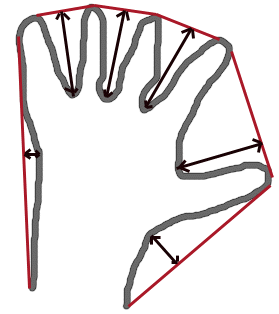
\includegraphics[width=0.5\textwidth]{pics/defects.png}

\cvCPyFunc{ContourArea}
Calculates the area of a whole contour or a contour section.

\cvdefC{
double cvContourArea( \par const CvArr* contour, \par CvSlice slice=CV\_WHOLE\_SEQ );
}
\cvdefPy{ContourArea(contour,slice=CV\_WHOLE\_SEQ)-> double}

\begin{description}
\cvarg{contour}{Contour (sequence or array of vertices)}
\cvarg{slice}{Starting and ending points of the contour section of interest, by default, the area of the whole contour is calculated}
\end{description}

The function calculates the area of a whole contour
or a contour section. In the latter case the total area bounded by the
contour arc and the chord connecting the 2 selected points is calculated
as shown on the picture below:

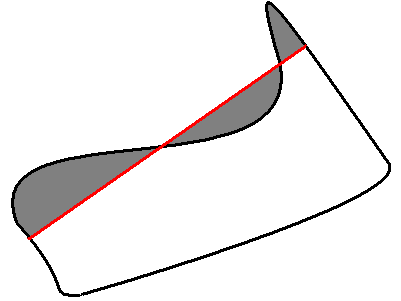
\includegraphics[width=0.5\textwidth]{pics/contoursecarea.png}

Orientation of the contour affects the area sign, thus the function may return a \emph{negative} result. Use the \texttt{fabs()} function from C runtime to get the absolute value of the area.

\cvCPyFunc{ContourFromContourTree}
Restores a contour from the tree.

\cvdefC{
CvSeq* cvContourFromContourTree( \par const CvContourTree* tree,\par CvMemStorage* storage,\par CvTermCriteria criteria );
}\cvdefPy{ContourFromContourTree(tree,storage,criteria)-> contour}

\begin{description}
\cvarg{tree}{Contour tree}
\cvarg{storage}{Container for the reconstructed contour}
\cvarg{criteria}{Criteria, where to stop reconstruction}
\end{description}

The function restores the contour from its binary tree representation. The parameter \texttt{criteria} determines the accuracy and/or the number of tree levels used for reconstruction, so it is possible to build an approximated contour. The function returns the reconstructed contour.

\cvCPyFunc{ConvexHull2}
Finds the convex hull of a point set.

\cvdefC{
CvSeq* cvConvexHull2( \par const CvArr* input,\par void* storage=NULL,\par int orientation=CV\_CLOCKWISE,\par int return\_points=0 );
}
\cvdefPy{ConvexHull2(points,storage,orientation=CV\_CLOCKWISE,return\_points=0)-> convex\_hull}

\begin{description}
\cvarg{points}{Sequence or array of 2D points with 32-bit integer or floating-point coordinates}
\cvarg{storage}{The destination array (CvMat*) or memory storage (CvMemStorage*) that will store the convex hull. If it is an array, it should be 1d and have the same number of elements as the input array/sequence. On output the header is modified as to truncate the array down to the hull size.  If \texttt{storage} is NULL then the convex hull will be stored in the same storage as the input sequence}
\cvarg{orientation}{Desired orientation of convex hull: \texttt{CV\_CLOCKWISE} or \texttt{CV\_COUNTER\_CLOCKWISE}}
\cvarg{return\_points}{If non-zero, the points themselves will be stored in the hull instead of indices if \texttt{storage} is an array, or pointers if \texttt{storage} is memory storage}
\end{description}

The function finds the convex hull of a 2D point set using Sklansky's algorithm. If \texttt{storage} is memory storage, the function creates a sequence containing the hull points or pointers to them, depending on \texttt{return\_points} value and returns the sequence on output.  If \texttt{storage} is a CvMat, the function returns NULL.

\ifC

Example. Building convex hull for a sequence or array of points

\begin{lstlisting}
#include "cv.h"
#include "highgui.h"
#include <stdlib.h>

#define ARRAY  0 /* switch between array/sequence method by replacing 0<=>1 */

void main( int argc, char** argv )
{
    IplImage* img = cvCreateImage( cvSize( 500, 500 ), 8, 3 );
    cvNamedWindow( "hull", 1 );

#if !ARRAY
        CvMemStorage* storage = cvCreateMemStorage();
#endif

    for(;;)
    {
        int i, count = rand()%100 + 1, hullcount;
        CvPoint pt0;
#if !ARRAY
        CvSeq* ptseq = cvCreateSeq( CV_SEQ_KIND_GENERIC|CV_32SC2,
                                    sizeof(CvContour),
                                    sizeof(CvPoint),
                                    storage );
        CvSeq* hull;

        for( i = 0; i < count; i++ )
        {
            pt0.x = rand() % (img->width/2) + img->width/4;
            pt0.y = rand() % (img->height/2) + img->height/4;
            cvSeqPush( ptseq, &pt0 );
        }
        hull = cvConvexHull2( ptseq, 0, CV_CLOCKWISE, 0 );
        hullcount = hull->total;
#else
        CvPoint* points = (CvPoint*)malloc( count * sizeof(points[0]));
        int* hull = (int*)malloc( count * sizeof(hull[0]));
        CvMat point_mat = cvMat( 1, count, CV_32SC2, points );
        CvMat hull_mat = cvMat( 1, count, CV_32SC1, hull );

        for( i = 0; i < count; i++ )
        {
            pt0.x = rand() % (img->width/2) + img->width/4;
            pt0.y = rand() % (img->height/2) + img->height/4;
            points[i] = pt0;
        }
        cvConvexHull2( &point_mat, &hull_mat, CV_CLOCKWISE, 0 );
        hullcount = hull_mat.cols;
#endif
        cvZero( img );
        for( i = 0; i < count; i++ )
        {
#if !ARRAY
            pt0 = *CV_GET_SEQ_ELEM( CvPoint, ptseq, i );
#else
            pt0 = points[i];
#endif
            cvCircle( img, pt0, 2, CV_RGB( 255, 0, 0 ), CV_FILLED );
        }

#if !ARRAY
        pt0 = **CV_GET_SEQ_ELEM( CvPoint*, hull, hullcount - 1 );
#else
        pt0 = points[hull[hullcount-1]];
#endif

        for( i = 0; i < hullcount; i++ )
        {
#if !ARRAY
            CvPoint pt = **CV_GET_SEQ_ELEM( CvPoint*, hull, i );
#else
            CvPoint pt = points[hull[i]];
#endif
            cvLine( img, pt0, pt, CV_RGB( 0, 255, 0 ));
            pt0 = pt;
        }

        cvShowImage( "hull", img );

        int key = cvWaitKey(0);
        if( key == 27 ) // 'ESC'
            break;

#if !ARRAY
        cvClearMemStorage( storage );
#else
        free( points );
        free( hull );
#endif
    }
}
\end{lstlisting}
\fi

\cvCPyFunc{ConvexityDefects}
Finds the convexity defects of a contour.

\cvdefC{
CvSeq* cvConvexityDefects( \par const CvArr* contour,\par const CvArr* convexhull,\par CvMemStorage* storage=NULL );
}\cvdefPy{ConvexityDefects(contour,convexhull,storage)-> convexity\_defects}

\begin{description}
\cvarg{contour}{Input contour}
\cvarg{convexhull}{Convex hull obtained using \cvCPyCross{ConvexHull2} that should contain pointers or indices to the contour points, not the hull points themselves (the \texttt{return\_points} parameter in \cvCPyCross{ConvexHull2} should be 0)}
\cvarg{storage}{Container for the output sequence of convexity defects. If it is NULL, the contour or hull (in that order) storage is used}
\end{description}

The function finds all convexity defects of the input contour and returns a sequence of the CvConvexityDefect structures.

\cvCPyFunc{CreateContourTree}
Creates a hierarchical representation of a contour.

\cvdefC{
CvContourTree* cvCreateContourTree( \par const CvSeq* contour,\par CvMemStorage* storage,\par double threshold );
}
\cvdefPy{CreateContourTree(contour,storage,threshold)-> contour\_tree}

\begin{description}
\cvarg{contour}{Input contour}
\cvarg{storage}{Container for output tree}
\cvarg{threshold}{Approximation accuracy}
\end{description}

The function creates a binary tree representation for the input \texttt{contour} and returns the pointer to its root. If the parameter \texttt{threshold} is less than or equal to 0, the function creates a full binary tree representation. If the threshold is greater than 0, the function creates a representation with the precision \texttt{threshold}: if the vertices with the interceptive area of its base line are less than \texttt{threshold}, the tree should not be built any further. The function returns the created tree.

\ifC % {

\cvCPyFunc{EndFindContours}
Finishes the scanning process.

\cvdefC{
CvSeq* cvEndFindContours( \par CvContourScanner* scanner );
}

\begin{description}
\cvarg{scanner}{Pointer to the contour scanner}
\end{description}

The function finishes the scanning process and returns a pointer to the first contour on the highest level.

\fi % }

\cvCPyFunc{FindContours}
Finds the contours in a binary image.

\cvdefC{
int cvFindContours(\par CvArr* image,\par CvMemStorage* storage,\par CvSeq** first\_contour,\par
                    int header\_size=sizeof(CvContour),\par int mode=CV\_RETR\_LIST,\par
                    int method=CV\_CHAIN\_APPROX\_SIMPLE,\par CvPoint offset=cvPoint(0,0) );
}
\cvdefPy{FindContours(image, storage, mode=CV\_RETR\_LIST, method=CV\_CHAIN\_APPROX\_SIMPLE, offset=(0,0)) -> cvseq}

\begin{description}
\cvarg{image}{The source, an 8-bit single channel image. Non-zero pixels are treated as 1's, zero pixels remain 0's - the image is treated as \texttt{binary}. To get such a binary image from grayscale, one may use \cvCPyCross{Threshold}, \cvCPyCross{AdaptiveThreshold} or \cvCPyCross{Canny}. The function modifies the source image's content}
\cvarg{storage}{Container of the retrieved contours}
\ifC
\cvarg{first\_contour}{Output parameter, will contain the pointer to the first outer contour}
\cvarg{header\_size}{Size of the sequence header, $\ge \texttt{sizeof(CvChain)}$ if $\texttt{method} =\texttt{CV\_CHAIN\_CODE}$,
and $\ge \texttt{sizeof(CvContour)}$ otherwise}
\fi
\cvarg{mode}{Retrieval mode
\begin{description}
  \cvarg{CV\_RETR\_EXTERNAL}{retrives only the extreme outer contours}
  \cvarg{CV\_RETR\_LIST}{retrieves all of the contours and puts them in the list}
  \cvarg{CV\_RETR\_CCOMP}{retrieves all of the contours and organizes them into a two-level hierarchy: on the top level are the external boundaries of the components, on the second level are the boundaries of the holes}
  \cvarg{CV\_RETR\_TREE}{retrieves all of the contours and reconstructs the full hierarchy of nested contours}
\end{description}}
\cvarg{method}{Approximation method (for all the modes, except \texttt{CV\_LINK\_RUNS}, which uses built-in approximation)
\begin{description}
  \cvarg{CV\_CHAIN\_CODE}{outputs contours in the Freeman chain code. All other methods output polygons (sequences of vertices)}
  \cvarg{CV\_CHAIN\_APPROX\_NONE}{translates all of the points from the chain code into points}
  \cvarg{CV\_CHAIN\_APPROX\_SIMPLE}{compresses horizontal, vertical, and diagonal segments and leaves only their end points}
  \cvarg{CV\_CHAIN\_APPROX\_TC89\_L1,CV\_CHAIN\_APPROX\_TC89\_KCOS}{applies one of the flavors of the Teh-Chin chain approximation algorithm.}
  \cvarg{CV\_LINK\_RUNS}{uses a completely different contour retrieval algorithm by linking horizontal segments of 1's. Only the \texttt{CV\_RETR\_LIST} retrieval mode can be used with this method.}
\end{description}}
\cvarg{offset}{Offset, by which every contour point is shifted. This is useful if the contours are extracted from the image ROI and then they should be analyzed in the whole image context}
\end{description}

The function retrieves contours from the binary image using the algorithm
\cite{Suzuki85}. The contours are a useful tool for shape analysis and
object detection and recognition.

The function retrieves contours from the
binary image and returns the number of retrieved contours. The
pointer \texttt{first\_contour} is filled by the function. It will
contain a pointer to the first outermost contour or \texttt{NULL} if no
contours are detected (if the image is completely black). Other
contours may be reached from \texttt{first\_contour} using the
\texttt{h\_next} and \texttt{v\_next} links. The sample in the
\cvCPyCross{DrawContours} discussion shows how to use contours for
connected component detection. Contours can be also used for shape
analysis and object recognition - see
\ifC
\texttt{squares.c}
\else
\texttt{squares.py}
\fi
in the OpenCV sample directory.

\textbf{Note:} the source \texttt{image} is modified by this function.

\ifC % {

\cvCPyFunc{FindNextContour}
Finds the next contour in the image.

\cvdefC{
CvSeq* cvFindNextContour( \par CvContourScanner scanner );
}

\begin{description}
\cvarg{scanner}{Contour scanner initialized by \cvCPyCross{StartFindContours} }
\end{description}

The function locates and retrieves the next contour in the image and returns a pointer to it. The function returns NULL if there are no more contours.

\fi % }

\cvCPyFunc{FitEllipse2}
Fits an ellipse around a set of 2D points.

\cvdefC{
CvBox2D cvFitEllipse2( \par const CvArr* points );
}
\cvdefPy{FitEllipse2(points)-> Box2D}

\begin{description}
\cvarg{points}{Sequence or array of points}
\end{description}

The function calculates the ellipse that fits best
(in least-squares sense) around a set of 2D points. The meaning of the
returned structure fields is similar to those in \cvCPyCross{Ellipse} except
that \texttt{size} stores the full lengths of the ellipse axises,
not half-lengths.

\cvCPyFunc{FitLine}
Fits a line to a 2D or 3D point set.

\cvdefC{
void  cvFitLine( \par const CvArr* points,\par int dist\_type,\par double param,\par double reps,\par double aeps,\par float* line );
}
\cvdefPy{FitLine(points, dist\_type, param, reps, aeps) -> line}

\begin{description}
\cvarg{points}{Sequence or array of 2D or 3D points with 32-bit integer or floating-point coordinates}
\cvarg{dist\_type}{The distance used for fitting (see the discussion)}
\cvarg{param}{Numerical parameter (\texttt{C}) for some types of distances, if 0 then some optimal value is chosen}
\cvarg{reps}{Sufficient accuracy for the radius (distance between the coordinate origin and the line).  0.01 is a good default value.}
\cvarg{aeps}{Sufficient accuracy for the angle.  0.01 is a good default value.}
\cvarg{line}{The output line parameters. In the case of a 2d fitting,
it is \cvC{an array} \cvPy{a tuple} of 4 floats \texttt{(vx, vy, x0, y0)} where \texttt{(vx, vy)} is a normalized vector collinear to the
line and \texttt{(x0, y0)} is some point on the line. in the case of a
3D fitting it is \cvC{an array} \cvPy{a tuple} of 6 floats \texttt{(vx, vy, vz, x0, y0, z0)}
where \texttt{(vx, vy, vz)} is a normalized vector collinear to the line
and \texttt{(x0, y0, z0)} is some point on the line}
\end{description}

The function fits a line to a 2D or 3D point set by minimizing $\sum_i \rho(r_i)$ where $r_i$ is the distance between the $i$ th point and the line and $\rho(r)$ is a distance function, one of:

\begin{description}

\item[dist\_type=CV\_DIST\_L2]
\[ \rho(r) = r^2/2 \quad \text{(the simplest and the fastest least-squares method)} \]

\item[dist\_type=CV\_DIST\_L1]
\[ \rho(r) = r \]

\item[dist\_type=CV\_DIST\_L12]
\[ \rho(r) = 2 \cdot (\sqrt{1 + \frac{r^2}{2}} - 1) \]

\item[dist\_type=CV\_DIST\_FAIR]
\[ \rho\left(r\right) = C^2 \cdot \left( \frac{r}{C} - \log{\left(1 + \frac{r}{C}\right)}\right) \quad \text{where} \quad C=1.3998 \]

\item[dist\_type=CV\_DIST\_WELSCH]
\[ \rho\left(r\right) = \frac{C^2}{2} \cdot \left( 1 - \exp{\left(-\left(\frac{r}{C}\right)^2\right)}\right) \quad \text{where} \quad C=2.9846 \]

\item[dist\_type=CV\_DIST\_HUBER]
\[ \rho(r) = \fork
{r^2/2}{if $r < C$}
{C \cdot (r-C/2)}{otherwise}  \quad \text{where} \quad C=1.345
\]
\end{description}

\cvCPyFunc{GetCentralMoment}
Retrieves the central moment from the moment state structure.

\cvdefC{
double cvGetCentralMoment( \par CvMoments* moments,\par int x\_order,\par int y\_order );
}
\cvdefPy{GetCentralMoment(moments, x\_order, y\_order) -> double}

\begin{description}
\cvarg{moments}{Pointer to the moment state structure}
\cvarg{x\_order}{x order of the retrieved moment, $\texttt{x\_order} >= 0$}
\cvarg{y\_order}{y order of the retrieved moment, $\texttt{y\_order} >= 0$ and $\texttt{x\_order} + \texttt{y\_order} <= 3$}
\end{description}

The function retrieves the central moment, which in the case of image moments is defined as:

\[
\mu_{x\_order, \, y\_order} = \sum_{x,y} (I(x,y) \cdot (x-x_c)^{x\_order} \cdot (y-y_c)^{y\_order})
\]

where $x_c,y_c$ are the coordinates of the gravity center:

\[
x_c=\frac{M_{10}}{M_{00}}, y_c=\frac{M_{01}}{M_{00}}
\]

\cvCPyFunc{GetHuMoments}
Calculates the seven Hu invariants.

\cvdefC{void cvGetHuMoments( const CvMoments* moments,CvHuMoments* hu );}
\cvdefPy{GetHuMoments(moments) -> hu}

\begin{description}
\cvarg{moments}{The input moments, computed with \cvCPyCross{Moments}}
\cvarg{hu}{The output Hu invariants}
\end{description}

The function calculates the seven Hu invariants, see \url{http://en.wikipedia.org/wiki/Image_moment}, that are defined as:

\[ \begin{array}{l}
hu_1=\eta_{20}+\eta_{02}\\
hu_2=(\eta_{20}-\eta_{02})^{2}+4\eta_{11}^{2}\\
hu_3=(\eta_{30}-3\eta_{12})^{2}+ (3\eta_{21}-\eta_{03})^{2}\\
hu_4=(\eta_{30}+\eta_{12})^{2}+ (\eta_{21}+\eta_{03})^{2}\\
hu_5=(\eta_{30}-3\eta_{12})(\eta_{30}+\eta_{12})[(\eta_{30}+\eta_{12})^{2}-3(\eta_{21}+\eta_{03})^{2}]+(3\eta_{21}-\eta_{03})(\eta_{21}+\eta_{03})[3(\eta_{30}+\eta_{12})^{2}-(\eta_{21}+\eta_{03})^{2}]\\
hu_6=(\eta_{20}-\eta_{02})[(\eta_{30}+\eta_{12})^{2}- (\eta_{21}+\eta_{03})^{2}]+4\eta_{11}(\eta_{30}+\eta_{12})(\eta_{21}+\eta_{03})\\
hu_7=(3\eta_{21}-\eta_{03})(\eta_{21}+\eta_{03})[3(\eta_{30}+\eta_{12})^{2}-(\eta_{21}+\eta_{03})^{2}]-(\eta_{30}-3\eta_{12})(\eta_{21}+\eta_{03})[3(\eta_{30}+\eta_{12})^{2}-(\eta_{21}+\eta_{03})^{2}]\\
\end{array}
\]

where $\eta_{ji}$ denote the normalized central moments.

These values are proved to be invariant to the image scale, rotation, and reflection except the seventh one, whose sign is changed by reflection. Of course, this invariance was proved with the assumption of infinite image resolution. In case of a raster images the computed Hu invariants for the original and transformed images will be a bit different.

\ifPy
\begin{lstlisting}
>>> import cv
>>> original = cv.LoadImageM("building.jpg", cv.CV_LOAD_IMAGE_GRAYSCALE)
>>> print cv.GetHuMoments(cv.Moments(original))
(0.0010620951868446141, 1.7962726159653835e-07, 1.4932744974469421e-11, 4.4832441315737963e-12, -1.0819359198251739e-23, -9.5726503811945833e-16, -3.5050592804744648e-23)
>>> flipped = cv.CloneMat(original)
>>> cv.Flip(original, flipped)
>>> print cv.GetHuMoments(cv.Moments(flipped))
(0.0010620951868446141, 1.796272615965384e-07, 1.4932744974469935e-11, 4.4832441315740249e-12, -1.0819359198259393e-23, -9.572650381193327e-16, 3.5050592804745877e-23)
\end{lstlisting}
\fi

\cvCPyFunc{GetNormalizedCentralMoment}
Retrieves the normalized central moment from the moment state structure.

\cvdefC{
double cvGetNormalizedCentralMoment( \par CvMoments* moments,\par int x\_order,\par int y\_order );
}\cvdefPy{GetNormalizedCentralMoment(moments, x\_order, y\_order) -> double}

\begin{description}
\cvarg{moments}{Pointer to the moment state structure}
\cvarg{x\_order}{x order of the retrieved moment, $\texttt{x\_order} >= 0$}
\cvarg{y\_order}{y order of the retrieved moment, $\texttt{y\_order} >= 0$ and $\texttt{x\_order} + \texttt{y\_order} <= 3$}
\end{description}

The function retrieves the normalized central moment:

\[
\eta_{x\_order, \, y\_order} = \frac{\mu_{x\_order, \, y\_order}}{M_{00}^{(y\_order+x\_order)/2+1}}
\]

\cvCPyFunc{GetSpatialMoment}
Retrieves the spatial moment from the moment state structure.

\cvdefC{
double cvGetSpatialMoment( \par CvMoments* moments, \par int x\_order, \par int y\_order );
}
\cvdefPy{GetSpatialMoment(moments, x\_order, y\_order) -> double}

\begin{description}
\cvarg{moments}{The moment state, calculated by \cvCPyCross{Moments}}
\cvarg{x\_order}{x order of the retrieved moment, $\texttt{x\_order} >= 0$}
\cvarg{y\_order}{y order of the retrieved moment, $\texttt{y\_order} >= 0$ and $\texttt{x\_order} + \texttt{y\_order} <= 3$}
\end{description}

The function retrieves the spatial moment, which in the case of image moments is defined as:

\[
M_{x\_order, \, y\_order} = \sum_{x,y} (I(x,y) \cdot x^{x\_order} \cdot y^{y\_order})
\]

where $I(x,y)$ is the intensity of the pixel $(x, y)$.

\cvCPyFunc{MatchContourTrees}
Compares two contours using their tree representations.

\cvdefC{
double cvMatchContourTrees( \par const CvContourTree* tree1,\par const CvContourTree* tree2,\par int method,\par double threshold );
}\cvdefPy{MatchContourTrees(tree1,tree2,method,threshold)-> double}

\begin{description}
\cvarg{tree1}{First contour tree}
\cvarg{tree2}{Second contour tree}
\cvarg{method}{Similarity measure, only \texttt{CV\_CONTOUR\_TREES\_MATCH\_I1} is supported}
\cvarg{threshold}{Similarity threshold}
\end{description}

The function calculates the value of the matching measure for two contour trees. The similarity measure is calculated level by level from the binary tree roots. If at a certain level the difference between contours becomes less than \texttt{threshold}, the reconstruction process is interrupted and the current difference is returned.

\cvCPyFunc{MatchShapes}
Compares two shapes.

\cvdefC{
double cvMatchShapes( \par const void* object1,\par const void* object2,\par int method,\par double parameter=0 );
}\cvdefPy{MatchShapes(object1,object2,method,parameter=0)-> None}

\begin{description}
\cvarg{object1}{First contour or grayscale image}
\cvarg{object2}{Second contour or grayscale image}
\cvarg{method}{Comparison method;
 \texttt{CV\_CONTOUR\_MATCH\_I1}, 
 \texttt{CV\_CONTOURS\_MATCH\_I2} 
or 
 \texttt{CV\_CONTOURS\_MATCH\_I3}}
\cvarg{parameter}{Method-specific parameter (is not used now)}
\end{description}

The function compares two shapes. The 3 implemented methods all use Hu moments (see \cvCPyCross{GetHuMoments}) ($A$ is \texttt{object1}, $B$ is \texttt{object2}):

\begin{description}
\item[method=CV\_CONTOUR\_MATCH\_I1]
\[ I_1(A,B) = \sum_{i=1...7} \left| \frac{1}{m^A_i} - \frac{1}{m^B_i} \right| \]

\item[method=CV\_CONTOUR\_MATCH\_I2]
\[ I_2(A,B) = \sum_{i=1...7} \left| m^A_i - m^B_i \right| \]

\item[method=CV\_CONTOUR\_MATCH\_I3]
\[ I_3(A,B) = \sum_{i=1...7} \frac{ \left| m^A_i - m^B_i \right| }{ \left| m^A_i \right| } \]
\end{description}

where

\[
\begin{array}{l}
m^A_i = sign(h^A_i) \cdot \log{h^A_i}
m^B_i = sign(h^B_i) \cdot \log{h^B_i}
\end{array}
\]

and $h^A_i, h^B_i$ are the Hu moments of $A$ and $B$ respectively.


\cvCPyFunc{MinAreaRect2}
Finds the circumscribed rectangle of minimal area for a given 2D point set.

\cvdefC{
CvBox2D  cvMinAreaRect2( \par const CvArr* points,\par CvMemStorage* storage=NULL );
}\cvdefPy{MinAreaRect2(points,storage=NULL)-> CvBox2D}

\begin{description}
\cvarg{points}{Sequence or array of points}
\cvarg{storage}{Optional temporary memory storage}
\end{description}

The function finds a circumscribed rectangle of the minimal area for a 2D point set by building a convex hull for the set and applying the rotating calipers technique to the hull.

Picture. Minimal-area bounding rectangle for contour

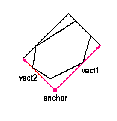
\includegraphics[width=0.5\textwidth]{pics/minareabox.png}

\cvCPyFunc{MinEnclosingCircle}
Finds the circumscribed circle of minimal area for a given 2D point set.

\cvdefC{
int cvMinEnclosingCircle( \par const CvArr* points,\par CvPoint2D32f* center,\par float* radius );
}
\cvdefPy{MinEnclosingCircle(points)-> (int,center,radius)}

\begin{description}
\cvarg{points}{Sequence or array of 2D points}
\cvarg{center}{Output parameter; the center of the enclosing circle}
\cvarg{radius}{Output parameter; the radius of the enclosing circle}
\end{description}

The function finds the minimal circumscribed
circle for a 2D point set using an iterative algorithm. It returns nonzero
if the resultant circle contains all the input points and zero otherwise
(i.e. the algorithm failed).

\cvCPyFunc{Moments}
Calculates all of the moments up to the third order of a polygon or rasterized shape.

\cvdefC{
void cvMoments( \par const CvArr* arr,\par CvMoments* moments,\par int binary=0 );
}
\cvdefPy{Moments(arr, binary = 0) -> moments}

\begin{description}
\cvarg{arr}{Image (1-channel or 3-channel with COI set) or polygon (CvSeq of points or a vector of points)}
\cvarg{moments}{Pointer to returned moment's state structure}
\cvarg{binary}{(For images only) If the flag is non-zero, all of the zero pixel values are treated as zeroes, and all of the others are treated as 1's}
\end{description}

The function calculates spatial and central moments up to the third order and writes them to \texttt{moments}. The moments may then be used then to calculate the gravity center of the shape, its area, main axises and various shape characeteristics including 7 Hu invariants.

\cvCPyFunc{PointPolygonTest}
Point in contour test.

\cvdefC{
double cvPointPolygonTest( \par const CvArr* contour,\par CvPoint2D32f pt,\par int measure\_dist );
}\cvdefPy{PointPolygonTest(contour,pt,measure\_dist)-> double}

\begin{description}
\cvarg{contour}{Input contour}
\cvarg{pt}{The point tested against the contour}
\cvarg{measure\_dist}{If it is non-zero, the function estimates the distance from the point to the nearest contour edge}
\end{description}

The function determines whether the
point is inside a contour, outside, or lies on an edge (or coinsides
with a vertex). It returns positive, negative or zero value,
correspondingly. When $\texttt{measure\_dist} =0$, the return value
is +1, -1 and 0, respectively. When $\texttt{measure\_dist} \ne 0$,
it is a signed distance between the point and the nearest contour
edge.

Here is the sample output of the function, where each image pixel is tested against the contour.

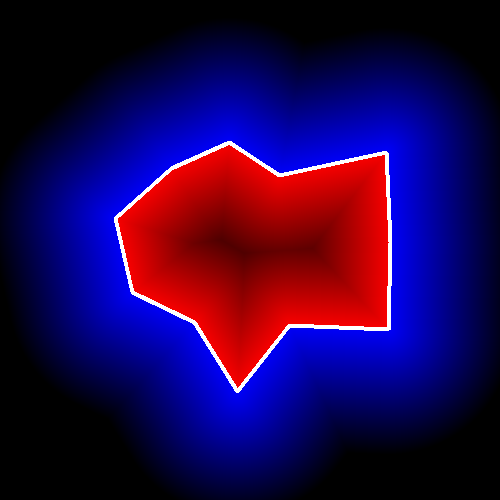
\includegraphics[width=0.5\textwidth]{pics/pointpolygon.png}

\ifC

\cvCPyFunc{PointSeqFromMat}
Initializes a point sequence header from a point vector.

\cvdefC{
CvSeq* cvPointSeqFromMat( \par int seq\_kind,\par const CvArr* mat,\par CvContour* contour\_header,\par CvSeqBlock* block );
}

\begin{description}
\cvarg{seq\_kind}{Type of the point sequence: point set (0), a curve (\texttt{CV\_SEQ\_KIND\_CURVE}), closed curve (\texttt{CV\_SEQ\_KIND\_CURVE+CV\_SEQ\_FLAG\_CLOSED}) etc.}
\cvarg{mat}{Input matrix. It should be a continuous, 1-dimensional vector of points, that is, it should have type \texttt{CV\_32SC2} or \texttt{CV\_32FC2}}
\cvarg{contour\_header}{Contour header, initialized by the function}
\cvarg{block}{Sequence block header, initialized by the function}
\end{description}

The function initializes a sequence
header to create a "virtual" sequence in which elements reside in
the specified matrix. No data is copied. The initialized sequence
header may be passed to any function that takes a point sequence
on input. No extra elements can be added to the sequence,
but some may be removed. The function is a specialized variant of
\cvCPyCross{MakeSeqHeaderForArray} and uses
the latter internally. It returns a pointer to the initialized contour
header. Note that the bounding rectangle (field \texttt{rect} of
\texttt{CvContour} strucuture) is not initialized by the function. If
you need one, use \cvCPyCross{BoundingRect}.

Here is a simple usage example.

\begin{lstlisting}
CvContour header;
CvSeqBlock block;
CvMat* vector = cvCreateMat( 1, 3, CV_32SC2 );

CV_MAT_ELEM( *vector, CvPoint, 0, 0 ) = cvPoint(100,100);
CV_MAT_ELEM( *vector, CvPoint, 0, 1 ) = cvPoint(100,200);
CV_MAT_ELEM( *vector, CvPoint, 0, 2 ) = cvPoint(200,100);

IplImage* img = cvCreateImage( cvSize(300,300), 8, 3 );
cvZero(img);

cvDrawContours( img,
    cvPointSeqFromMat(CV_SEQ_KIND_CURVE+CV_SEQ_FLAG_CLOSED,
                      vector,
                      &header,
                      &block),
                CV_RGB(255,0,0),
                CV_RGB(255,0,0),
                0, 3, 8, cvPoint(0,0));
\end{lstlisting}


\cvCPyFunc{ReadChainPoint}
Gets the next chain point.

\cvdefC{
CvPoint cvReadChainPoint( CvChainPtReader* reader );
}

\begin{description}
\cvarg{reader}{Chain reader state}
\end{description}

The function returns the current chain point and updates the reader position.

\cvCPyFunc{StartFindContours}
Initializes the contour scanning process.

\cvdefC{
CvContourScanner cvStartFindContours(\par CvArr* image,\par CvMemStorage* storage,\par
                                      int header\_size=sizeof(CvContour),\par
                                      int mode=CV\_RETR\_LIST,\par
                                      int method=CV\_CHAIN\_APPROX\_SIMPLE,\par
                                      CvPoint offset=cvPoint(0,\par0) );
}

\begin{description}
\cvarg{image}{The 8-bit, single channel, binary source image}
\cvarg{storage}{Container of the retrieved contours}
\cvarg{header\_size}{Size of the sequence header, $>=sizeof(CvChain)$ if \texttt{method} =CV\_CHAIN\_CODE, and $>=sizeof(CvContour)$ otherwise}
\cvarg{mode}{Retrieval mode; see \cvCPyCross{FindContours}}
\cvarg{method}{Approximation method. It has the same meaning in \cvCPyCross{FindContours}, but \texttt{CV\_LINK\_RUNS} can not be used here}
\cvarg{offset}{ROI offset; see \cvCPyCross{FindContours}}
\end{description}

The function initializes and returns a pointer to the contour scanner. The scanner is used in \cvCPyCross{FindNextContour} to retrieve the rest of the contours.

\cvCPyFunc{StartReadChainPoints}
Initializes the chain reader.

\cvdefC{
void cvStartReadChainPoints( CvChain* chain, CvChainPtReader* reader );
}

The function initializes a special reader.

\cvCPyFunc{SubstituteContour}
Replaces a retrieved contour.

\cvdefC{
void cvSubstituteContour( \par CvContourScanner scanner, \par CvSeq* new\_contour );
}

\begin{description}
\cvarg{scanner}{Contour scanner initialized by \cvCPyCross{StartFindContours} }
\cvarg{new\_contour}{Substituting contour}
\end{description}

The function replaces the retrieved
contour, that was returned from the preceding call of
\cvCPyCross{FindNextContour} and stored inside the contour scanner
state, with the user-specified contour. The contour is inserted
into the resulting structure, list, two-level hierarchy, or tree,
depending on the retrieval mode. If the parameter \texttt{new\_contour}
is \texttt{NULL}, the retrieved contour is not included in the
resulting structure, nor are any of its children that might be added
to this structure later.

\fi

\fi


\ifCpp

\cvCppFunc{moments}
Calculates all of the moments up to the third order of a polygon or rasterized shape.

\cvdefCpp{Moments moments( const Mat\& array, bool binaryImage=false );}

where the class \texttt{Moments} is defined as:
\begin{lstlisting}
class Moments
{
public:
    Moments();
    Moments(double m00, double m10, double m01, double m20, double m11,
            double m02, double m30, double m21, double m12, double m03 );
    Moments( const CvMoments\& moments );
    operator CvMoments() const;
    
    // spatial moments
    double  m00, m10, m01, m20, m11, m02, m30, m21, m12, m03;
    // central moments
    double  mu20, mu11, mu02, mu30, mu21, mu12, mu03;
    // central normalized moments
    double  nu20, nu11, nu02, nu30, nu21, nu12, nu03;
};
\end{lstlisting}

\begin{description}
\cvarg{array}{A raster image (single-channel, 8-bit or floating-point 2D array) or an array
    ($1 \times N$ or $N \times 1$) of 2D points (\texttt{Point} or \texttt{Point2f})}
\cvarg{binaryImage}{(For images only) If it is true, then all the non-zero image pixels are treated as 1's}
\end{description}

The function computes moments, up to the 3rd order, of a vector shape or a rasterized shape.
In case of a raster image, the spatial moments $\texttt{Moments::m}_{ji}$ are computed as:

\[\texttt{m}_{ji}=\sum_{x,y} \left(\texttt{array}(x,y) \cdot x^j \cdot y^i\right),\]

the central moments $\texttt{Moments::mu}_{ji}$ are computed as:
\[\texttt{mu}_{ji}=\sum_{x,y} \left(\texttt{array}(x,y) \cdot (x - \bar{x})^j \cdot (y - \bar{y})^i\right)\]
where $(\bar{x}, \bar{y})$ is the mass center:

\[
\bar{x}=\frac{\texttt{m}_{10}}{\texttt{m}_{00}},\; \bar{y}=\frac{\texttt{m}_{01}}{\texttt{m}_{00}}
\]

and the normalized central moments $\texttt{Moments::nu}_{ij}$ are computed as:
\[\texttt{nu}_{ji}=\frac{\texttt{mu}_{ji}}{\texttt{m}_{00}^{(i+j)/2+1}}.\]

Note that $\texttt{mu}_{00}=\texttt{m}_{00}$, $\texttt{nu}_{00}=1$ $\texttt{nu}_{10}=\texttt{mu}_{10}=\texttt{mu}_{01}=\texttt{mu}_{10}=0$, hence the values are not stored.

The moments of a contour are defined in the same way, but computed using Green's formula
(see \url{http://en.wikipedia.org/wiki/Green_theorem}), therefore, because of a limited raster resolution, the moments computed for a contour will be slightly different from the moments computed for the same contour rasterized.

See also: \cvCppCross{contourArea}, \cvCppCross{arcLength}

\cvCppFunc{HuMoments}
Calculates the seven Hu invariants.

\cvdefCpp{void HuMoments( const Moments\& moments, double h[7] );}
\begin{description}
\cvarg{moments}{The input moments, computed with \cvCppCross{moments}}
\cvarg{h}{The output Hu invariants}
\end{description}

The function calculates the seven Hu invariants, see \url{http://en.wikipedia.org/wiki/Image_moment}, that are defined as:

\[ \begin{array}{l}
h[0]=\eta_{20}+\eta_{02}\\
h[1]=(\eta_{20}-\eta_{02})^{2}+4\eta_{11}^{2}\\
h[2]=(\eta_{30}-3\eta_{12})^{2}+ (3\eta_{21}-\eta_{03})^{2}\\
h[3]=(\eta_{30}+\eta_{12})^{2}+ (\eta_{21}+\eta_{03})^{2}\\
h[4]=(\eta_{30}-3\eta_{12})(\eta_{30}+\eta_{12})[(\eta_{30}+\eta_{12})^{2}-3(\eta_{21}+\eta_{03})^{2}]+(3\eta_{21}-\eta_{03})(\eta_{21}+\eta_{03})[3(\eta_{30}+\eta_{12})^{2}-(\eta_{21}+\eta_{03})^{2}]\\
h[5]=(\eta_{20}-\eta_{02})[(\eta_{30}+\eta_{12})^{2}- (\eta_{21}+\eta_{03})^{2}]+4\eta_{11}(\eta_{30}+\eta_{12})(\eta_{21}+\eta_{03})\\
h[6]=(3\eta_{21}-\eta_{03})(\eta_{21}+\eta_{03})[3(\eta_{30}+\eta_{12})^{2}-(\eta_{21}+\eta_{03})^{2}]-(\eta_{30}-3\eta_{12})(\eta_{21}+\eta_{03})[3(\eta_{30}+\eta_{12})^{2}-(\eta_{21}+\eta_{03})^{2}]\\
\end{array}
\]

where $\eta_{ji}$ stand for $\texttt{Moments::nu}_{ji}$.

These values are proved to be invariant to the image scale, rotation, and reflection except the seventh one, whose sign is changed by reflection. Of course, this invariance was proved with the assumption of infinite image resolution. In case of a raster images the computed Hu invariants for the original and transformed images will be a bit different.

See also: \cvCppCross{matchShapes}

\cvCppFunc{findContours}
Finds the contours in a binary image.

\cvdefCpp{void findContours( const Mat\& image, vector<vector<Point> >\& contours,\par
                   vector<Vec4i>\& hierarchy, int mode,\par
                   int method, Point offset=Point());\newline
void findContours( const Mat\& image, vector<vector<Point> >\& contours,\par
                   int mode, int method, Point offset=Point());
}
\begin{description}
\cvarg{image}{The source, an 8-bit single-channel image. Non-zero pixels are treated as 1's, zero pixels remain 0's - the image is treated as \texttt{binary}. You can use \cvCppCross{compare}, \cvCppCross{inRange}, \cvCppCross{threshold}, \cvCppCross{adaptiveThreshold}, \cvCppCross{Canny} etc. to create a binary image out of a grayscale or color one. The function modifies the \texttt{image} while extracting the contours}
\cvarg{contours}{The detected contours. Each contour is stored as a vector of points}
\cvarg{hiararchy}{The optional output vector that will contain information about the image topology. It will have as many elements as the number of contours. For each contour \texttt{contours[i]}, the elements \texttt{hierarchy[i][0]}, \texttt{hiearchy[i][1]}, \texttt{hiearchy[i][2]}, \texttt{hiearchy[i][3]} will be set to 0-based indices in \texttt{contours} of the next and previous contours at the same hierarchical level, the first child contour and the parent contour, respectively. If for some contour \texttt{i} there is no next, previous, parent or nested contours, the corresponding elements of \texttt{hierarchy[i]} will be negative}
\cvarg{mode}{The contour retrieval mode
\begin{description}
  \cvarg{CV\_RETR\_EXTERNAL}{retrieves only the extreme outer contours; It will set \texttt{hierarchy[i][2]=hierarchy[i][3]=-1} for all the contours}
  \cvarg{CV\_RETR\_LIST}{retrieves all of the contours without establishing any hierarchical relationships}
  \cvarg{CV\_RETR\_CCOMP}{retrieves all of the contours and organizes them into a two-level hierarchy: on the top level are the external boundaries of the components, on the second level are the boundaries of the holes. If inside a hole of a connected component there is another contour, it will still be put on the top level}
  \cvarg{CV\_RETR\_TREE}{retrieves all of the contours and reconstructs the full hierarchy of nested contours. This full hierarchy is built and shown in OpenCV \texttt{contours.c} demo}
\end{description}}
\cvarg{method}{The contour approximation method.
\begin{description}
  \cvarg{CV\_CHAIN\_APPROX\_NONE}{stores absolutely all the contour points. That is, every 2 points of a contour stored with this method are 8-connected neighbors of each other}
  \cvarg{CV\_CHAIN\_APPROX\_SIMPLE}{compresses horizontal, vertical, and diagonal segments and leaves only their end points. E.g. an up-right rectangular contour will be encoded with 4 points}
  \cvarg{CV\_CHAIN\_APPROX\_TC89\_L1,CV\_CHAIN\_APPROX\_TC89\_KCOS}{applies one of the flavors of the Teh-Chin chain approximation algorithm; see \cite{TehChin89}}
\end{description}}
\cvarg{offset}{The optional offset, by which every contour point is shifted. This is useful if the contours are extracted from the image ROI and then they should be analyzed in the whole image context}
\end{description}

The function retrieves contours from the
binary image using the algorithm \cite{Suzuki85}. The contours are a useful tool for shape analysis and object detection and recognition. See \texttt{squares.c} in the OpenCV sample directory.

\textbf{Note:} the source \texttt{image} is modified by this function.

\cvCppFunc{drawContours}
Draws contours' outlines or filled contours.

\cvdefCpp{void drawContours( Mat\& image, const vector<vector<Point> >\& contours,\par
                   int contourIdx, const Scalar\& color, int thickness=1,\par
                   int lineType=8, const vector<Vec4i>\& hierarchy=vector<Vec4i>(),\par
                   int maxLevel=INT\_MAX, Point offset=Point() );}
\begin{description}
\cvarg{image}{The destination image}
\cvarg{contours}{All the input contours. Each contour is stored as a point vector}
\cvarg{contourIdx}{Indicates the contour to draw. If it is negative, all the contours are drawn}
\cvarg{color}{The contours' color}
\cvarg{thickness}{Thickness of lines the contours are drawn with.
If it is negative (e.g. \texttt{thickness=CV\_FILLED}), the contour interiors are
drawn.}
\cvarg{lineType}{The line connectivity; see \cvCppCross{line} description}
\cvarg{hierarchy}{The optional information about hierarchy. It is only needed if you want to draw only some of the  contours (see \texttt{maxLevel})}
\cvarg{maxLevel}{Maximal level for drawn contours. If 0, only
the specified contour is drawn. If 1, the function draws the contour(s) and all the nested contours. If 2, the function draws the contours, all the nested contours and all the nested into nested contours etc. This parameter is only taken into account when there is \texttt{hierarchy} available.}
\cvarg{offset}{The optional contour shift parameter. Shift all the drawn contours by the specified $\texttt{offset}=(dx,dy)$}
\end{description}

The function draws contour outlines in the image if $\texttt{thickness} \ge 0$ or fills the area bounded by the contours if $ \texttt{thickness}<0$. Here is the example on how to retrieve connected components from the binary image and label them

\begin{lstlisting}
#include "cv.h"
#include "highgui.h"

using namespace cv;

int main( int argc, char** argv )
{
    Mat src;
    // the first command line parameter must be file name of binary 
    // (black-n-white) image
    if( argc != 2 || !(src=imread(argv[1], 0)).data)
        return -1;

    Mat dst = Mat::zeros(src.rows, src.cols, CV_8UC3);

    src = src > 1;
    namedWindow( "Source", 1 );
    imshow( "Source", src );

    vector<vector<Point> > contours;
    vector<Vec4i> hierarchy;
    
    findContours( src, contours, hierarchy, 
        CV_RETR_CCOMP, CV_CHAIN_APPROX_SIMPLE );

    // iterate through all the top-level contours,
    // draw each connected component with its own random color
    int idx = 0;
    for( ; idx >= 0; idx = hierarchy[idx][0] )
    {
        Scalar color( rand()&255, rand()&255, rand()&255 );
        drawContours( dst, contours, idx, color, CV_FILLED, 8, hierarchy );
    }

    namedWindow( "Components", 1 );
    imshow( "Components", dst );
    waitKey(0);
}
\end{lstlisting}


\cvCppFunc{approxPolyDP}
Approximates polygonal curve(s) with the specified precision.

\cvdefCpp{void approxPolyDP( const Mat\& curve,\par
                   vector<Point>\& approxCurve,\par
                   double epsilon, bool closed );\newline
void approxPolyDP( const Mat\& curve,\par
                   vector<Point2f>\& approxCurve,\par
                   double epsilon, bool closed );}
\begin{description}
\cvarg{curve}{The polygon or curve to approximate. Must be $1 \times N$ or $N \times 1$ matrix of type \texttt{CV\_32SC2} or \texttt{CV\_32FC2}. You can also convert \texttt{vector<Point>} or \texttt{vector<Point2f} to the matrix by calling \texttt{Mat(const vector<T>\&)} constructor.}
\cvarg{approxCurve}{The result of the approximation; The type should match the type of the input curve}
\cvarg{epsilon}{Specifies the approximation accuracy. This is the maximum distance between the original curve and its approximation}
\cvarg{closed}{If true, the approximated curve is closed (i.e. its first and last vertices are connected), otherwise it's not}
\end{description}

The functions \texttt{approxPolyDP} approximate a curve or a polygon with another curve/polygon with less vertices, so that the distance between them is less or equal to the specified precision. It used Douglas-Peucker algorithm \url{http://en.wikipedia.org/wiki/Ramer-Douglas-Peucker_algorithm}

\cvCppFunc{arcLength}
Calculates a contour perimeter or a curve length.

\cvdefCpp{double arcLength( const Mat\& curve, bool closed );}
\begin{description}
\cvarg{curve}{The input vector of 2D points, represented by \texttt{CV\_32SC2} or \texttt{CV\_32FC2} matrix, or by \texttt{vector<Point>} or \texttt{vector<Point2f>} converted to a matrix with \texttt{Mat(const vector<T>\&)} constructor}
\cvarg{closed}{Indicates, whether the curve is closed or not}
\end{description}

The function computes the curve length or the closed contour perimeter.

\cvCppFunc{boundingRect}
Calculates the up-right bounding rectangle of a point set.

\cvdefCpp{Rect boundingRect( const Mat\& points );}
\begin{description}
\cvarg{points}{The input 2D point set, represented by \texttt{CV\_32SC2} or \texttt{CV\_32FC2} matrix, or by \texttt{vector<Point>} or \texttt{vector<Point2f>} converted to the matrix using \texttt{Mat(const vector<T>\&)} constructor.}
\end{description}

The function calculates and returns the minimal up-right bounding rectangle for the specified point set.


\cvCppFunc{estimateRigidTransform}
Computes optimal affine transformation between two 2D point sets

\cvdefCpp{Mat estimateRigidTransform( const Mat\& srcpt, const Mat\& dstpt,\par
                            bool fullAffine );}
\begin{description}
\cvarg{srcpt}{The first input 2D point set}
\cvarg{dst}{The second input 2D point set of the same size and the same type as \texttt{A}}
\cvarg{fullAffine}{If true, the function finds the optimal affine transformation with no any additional resrictions (i.e. there are 6 degrees of freedom); otherwise, the class of transformations to choose from is limited to combinations of translation, rotation and uniform scaling (i.e. there are 5 degrees of freedom)}
\end{description}

The function finds the optimal affine transform $[A|b]$ (a $2 \times 3$ floating-point matrix) that approximates best the transformation from $\texttt{srcpt}_i$ to $\texttt{dstpt}_i$:

\[ [A^*|b^*] = arg \min_{[A|b]} \sum_i \|\texttt{dstpt}_i - A {\texttt{srcpt}_i}^T - b \|^2 \]

where $[A|b]$ can be either arbitrary (when \texttt{fullAffine=true}) or have form
\[\begin{bmatrix}a_{11} & a_{12} & b_1 \\ -a_{12} & a_{11} & b_2 \end{bmatrix}\] when \texttt{fullAffine=false}.

See also: \cvCppCross{getAffineTransform}, \cvCppCross{getPerspectiveTransform}, \cvCppCross{findHomography}

\cvCppFunc{estimateAffine3D}
Computes optimal affine transformation between two 3D point sets

\cvdefCpp{int estimateAffine3D(const Mat\& srcpt, const Mat\& dstpt, Mat\& out,\par
                     vector<uchar>\& outliers,\par
                     double ransacThreshold = 3.0,\par
                     double confidence = 0.99);}
\begin{description}
\cvarg{srcpt}{The first input 3D point set}
\cvarg{dstpt}{The second input 3D point set}
\cvarg{out}{The output 3D affine transformation matrix $3 \times 4$}
\cvarg{outliers}{The output vector indicating which points are outliers}
\cvarg{ransacThreshold}{The maximum reprojection error in RANSAC algorithm to consider a point an inlier}
\cvarg{confidence}{The confidence level, between 0 and 1, with which the matrix is estimated}
\end{description}

The function estimates the optimal 3D affine transformation between two 3D point sets using RANSAC algorithm.


\cvCppFunc{contourArea}
Calculates the contour area

\cvdefCpp{double contourArea( const Mat\& contour );    }
\begin{description}
\cvarg{contour}{The contour vertices, represented by \texttt{CV\_32SC2} or \texttt{CV\_32FC2} matrix, or by \texttt{vector<Point>} or \texttt{vector<Point2f>} converted to the matrix using \texttt{Mat(const vector<T>\&)} constructor.}
\end{description}

The function computes the contour area. Similarly to \cvCppCross{moments} the area is computed using the Green formula, thus the returned area and the number of non-zero pixels, if you draw the contour using \cvCppCross{drawContours} or \cvCppCross{fillPoly}, can be different.
Here is a short example:

\begin{lstlisting}
vector<Point> contour;
contour.push_back(Point2f(0, 0));
contour.push_back(Point2f(10, 0));
contour.push_back(Point2f(10, 10));
contour.push_back(Point2f(5, 4));

double area0 = contourArea(contour);
vector<Point> approx;
approxPolyDP(contour, approx, 5, true);
double area1 = contourArea(approx);

cout << "area0 =" << area0 << endl <<
        "area1 =" << area1 << endl <<
        "approx poly vertices" << approx.size() << endl; 
\end{lstlisting}

\cvCppFunc{convexHull}    
Finds the convex hull of a point set.

\cvdefCpp{void convexHull( const Mat\& points, vector<int>\& hull,\par
                 bool clockwise=false );\newline
void convexHull( const Mat\& points, vector<Point>\& hull,\par
                 bool clockwise=false );\newline
void convexHull( const Mat\& points, vector<Point2f>\& hull,\par
                 bool clockwise=false );}
\begin{description}
\cvarg{points}{The input 2D point set, represented by \texttt{CV\_32SC2} or \texttt{CV\_32FC2} matrix, or by \texttt{vector<Point>} or \texttt{vector<Point2f>} converted to the matrix using \texttt{Mat(const vector<T>\&)} constructor.}
\cvarg{hull}{The output convex hull. It is either a vector of points that form the hull (must have the same type as the input points), or a vector of 0-based point indices of the hull points in the original array (since the set of convex hull points is a subset of the original point set).}
\cvarg{clockwise}{If true, the output convex hull will be oriented clockwise, otherwise it will be oriented counter-clockwise. Here, the usual screen coordinate system is assumed - the origin is at the top-left corner, x axis is oriented to the right, and y axis is oriented downwards.}
\end{description}

The functions find the convex hull of a 2D point set using Sklansky's algorithm \cite{Sklansky82} that has $O(N logN)$ or $O(N)$ complexity (where $N$ is the number of input points), depending on how the initial sorting is implemented (currently it is $O(N logN)$. See the OpenCV sample \texttt{convexhull.c} that demonstrates the use of the different function variants. 


\cvCppFunc{fitEllipse}
Fits an ellipse around a set of 2D points.

\cvdefCpp{RotatedRect fitEllipse( const Mat\& points );}
\begin{description}
\cvarg{points}{The input 2D point set, represented by \texttt{CV\_32SC2} or \texttt{CV\_32FC2} matrix, or by \texttt{vector<Point>} or \texttt{vector<Point2f>} converted to the matrix using \texttt{Mat(const vector<T>\&)} constructor.}
\end{description}

The function calculates the ellipse that fits best
(in least-squares sense) a set of 2D points. It returns the rotated rectangle in which the ellipse is inscribed.

\cvCppFunc{fitLine}
Fits a line to a 2D or 3D point set.

\cvdefCpp{void fitLine( const Mat\& points, Vec4f\& line, int distType,\par
              double param, double reps, double aeps );\newline
void fitLine( const Mat\& points, Vec6f\& line, int distType,\par
              double param, double reps, double aeps );}
\begin{description}
\cvarg{points}{The input 2D point set, represented by \texttt{CV\_32SC2} or \texttt{CV\_32FC2} matrix, or by
\texttt{vector<Point>}, \texttt{vector<Point2f>}, \texttt{vector<Point3i>} or \texttt{vector<Point3f>} converted to the matrix by \texttt{Mat(const vector<T>\&)} constructor}
\cvarg{line}{The output line parameters. In the case of a 2d fitting,
it is a vector of 4 floats \texttt{(vx, vy,
x0, y0)} where \texttt{(vx, vy)} is a normalized vector collinear to the
line and \texttt{(x0, y0)} is some point on the line. in the case of a
3D fitting it is vector of 6 floats \texttt{(vx, vy, vz, x0, y0, z0)}
where \texttt{(vx, vy, vz)} is a normalized vector collinear to the line
and \texttt{(x0, y0, z0)} is some point on the line}
\cvarg{distType}{The distance used by the M-estimator (see the discussion)}
\cvarg{param}{Numerical parameter (\texttt{C}) for some types of distances, if 0 then some optimal value is chosen}
\cvarg{reps, aeps}{Sufficient accuracy for the radius (distance between the coordinate origin and the line) and angle, respectively; 0.01 would be a good default value for both.}
\end{description}

The functions \texttt{fitLine} fit a line to a 2D or 3D point set by minimizing $\sum_i \rho(r_i)$ where $r_i$ is the distance between the $i^{th}$ point and the line and $\rho(r)$ is a distance function, one of:

\begin{description}
\item[distType=CV\_DIST\_L2]
\[ \rho(r) = r^2/2 \quad \text{(the simplest and the fastest least-squares method)} \]

\item[distType=CV\_DIST\_L1]
\[ \rho(r) = r \]

\item[distType=CV\_DIST\_L12]
\[ \rho(r) = 2 \cdot (\sqrt{1 + \frac{r^2}{2}} - 1) \]

\item[distType=CV\_DIST\_FAIR]
\[ \rho\left(r\right) = C^2 \cdot \left( \frac{r}{C} - \log{\left(1 + \frac{r}{C}\right)}\right) \quad \text{where} \quad C=1.3998 \]

\item[distType=CV\_DIST\_WELSCH]
\[ \rho\left(r\right) = \frac{C^2}{2} \cdot \left( 1 - \exp{\left(-\left(\frac{r}{C}\right)^2\right)}\right) \quad \text{where} \quad C=2.9846 \]

\item[distType=CV\_DIST\_HUBER]
\[ \rho(r) = \fork
{r^2/2}{if $r < C$}
{C \cdot (r-C/2)}{otherwise}  \quad \text{where} \quad C=1.345
\]
\end{description}

The algorithm is based on the M-estimator (\url{http://en.wikipedia.org/wiki/M-estimator}) technique, that iteratively fits the line using weighted least-squares algorithm and after each iteration the weights $w_i$ are adjusted to beinversely proportional to $\rho(r_i)$. 


\cvCppFunc{isContourConvex}
Tests contour convexity.

\cvdefCpp{bool isContourConvex( const Mat\& contour );}
\begin{description}
\cvarg{contour}{The tested contour, a matrix of type \texttt{CV\_32SC2} or \texttt{CV\_32FC2}, or \texttt{vector<Point>} or \texttt{vector<Point2f>} converted to the matrix using \texttt{Mat(const vector<T>\&)} constructor.}
\end{description}

The function tests whether the input contour is convex or not. The contour must be simple, i.e. without self-intersections, otherwise the function output is undefined.


\cvCppFunc{minAreaRect}
Finds the minimum area rotated rectangle enclosing a 2D point set.

\cvdefCpp{RotatedRect minAreaRect( const Mat\& points );}
\begin{description}
\cvarg{points}{The input 2D point set, represented by \texttt{CV\_32SC2} or \texttt{CV\_32FC2} matrix, or by \texttt{vector<Point>} or \texttt{vector<Point2f>} converted to the matrix using \texttt{Mat(const vector<T>\&)} constructor.}
\end{description}

The function calculates and returns the minimum area bounding rectangle (possibly rotated) for the specified point set. See the OpenCV sample \texttt{minarea.c}

\cvCppFunc{minEnclosingCircle}
Finds the minimum area circle enclosing a 2D point set.

\cvdefCpp{void minEnclosingCircle( const Mat\& points, Point2f\& center, float\& radius );    }
\begin{description}
\cvarg{points}{The input 2D point set, represented by \texttt{CV\_32SC2} or \texttt{CV\_32FC2} matrix, or by \texttt{vector<Point>} or \texttt{vector<Point2f>} converted to the matrix using \texttt{Mat(const vector<T>\&)} constructor.}
\cvarg{center}{The output center of the circle}
\cvarg{radius}{The output radius of the circle}
\end{description}

The function finds the minimal enclosing circle of a 2D point set using iterative algorithm. See the OpenCV sample \texttt{minarea.c}

\cvCppFunc{matchShapes}
Compares two shapes.

\cvdefCpp{double matchShapes( const Mat\& object1,\par
                    const Mat\& object2,\par
                    int method, double parameter=0 );}
\begin{description}
\cvarg{object1}{The first contour or grayscale image}
\cvarg{object2}{The second contour or grayscale image}
\cvarg{method}{Comparison method:
 \texttt{CV\_CONTOUR\_MATCH\_I1},\\ 
 \texttt{CV\_CONTOURS\_MATCH\_I2}\\ 
or 
 \texttt{CV\_CONTOURS\_MATCH\_I3} (see the discussion below)}
\cvarg{parameter}{Method-specific parameter (is not used now)}
\end{description}

The function compares two shapes. The 3 implemented methods all use Hu invariants (see \cvCppCross{HuMoments}) as following ($A$ denotes \texttt{object1}, $B$ denotes \texttt{object2}):

\begin{description}
\item[method=CV\_CONTOUR\_MATCH\_I1]
\[ I_1(A,B) = \sum_{i=1...7} \left| \frac{1}{m^A_i} - \frac{1}{m^B_i} \right| \]

\item[method=CV\_CONTOUR\_MATCH\_I2]
\[ I_2(A,B) = \sum_{i=1...7} \left| m^A_i - m^B_i \right| \]

\item[method=CV\_CONTOUR\_MATCH\_I3]
\[ I_3(A,B) = \sum_{i=1...7} \frac{ \left| m^A_i - m^B_i \right| }{ \left| m^A_i \right| } \]
\end{description}

where

\[
\begin{array}{l}
m^A_i = \mathrm{sign}(h^A_i) \cdot \log{h^A_i} \\
m^B_i = \mathrm{sign}(h^B_i) \cdot \log{h^B_i}
\end{array}
\]

and $h^A_i, h^B_i$ are the Hu moments of $A$ and $B$ respectively.


\cvCppFunc{pointPolygonTest}
Performs point-in-contour test.

\cvdefCpp{double pointPolygonTest( const Mat\& contour,\par
                         Point2f pt, bool measureDist );}
\begin{description}
\cvarg{contour}{The input contour}
\cvarg{pt}{The point tested against the contour}
\cvarg{measureDist}{If true, the function estimates the signed distance from the point to the nearest contour edge; otherwise, the function only checks if the point is inside or not.}
\end{description}

The function determines whether the
point is inside a contour, outside, or lies on an edge (or coincides
with a vertex). It returns positive (inside), negative (outside) or zero (on an edge) value,
correspondingly. When \texttt{measureDist=false}, the return value
is +1, -1 and 0, respectively. Otherwise, the return value
it is a signed distance between the point and the nearest contour
edge.

Here is the sample output of the function, where each image pixel is tested against the contour.

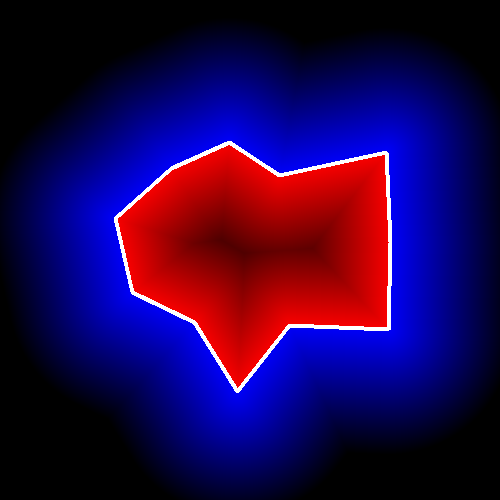
\includegraphics[width=0.5\textwidth]{pics/pointpolygon.png}

\fi
